\title{Spectator Attendance}
\label{Spectator_Attendance}

\section{Introduction}

In many team sports, the home-field advantage has a positive effect on the success of the home team \cite{cross2020fans, angelini2019efficiency, pollard2005long}. In particular, the effect of spectators with their supportive chants appears to influence the performance of the home team \cite{ponzo2018does}. For example, spectators have been shown to induce a referee bias that can lead referees to favor the home team \cite{dohmen2016referee, leitner2021no}. Due to the COVID-19 pandemic, spectator attendance in professional European football has been banned or limited for most games from March 2020 to the end of the 2021/2022 season. Since ghost games (games without spectators) were a rare phenomenon prior to the COVID-19 outbreak, the pandemic provided a unique opportunity to examine the impact of spectator attendance on home-field advantage in a natural experiment \cite{cueva2020animal}. By conducting this natural experiment and distinguishing games with and without spectators on outcome variables relevant to a team's success, causal inferences can be obtained \cite{jimenez2021home}.

A recent literature review by Leitner et al. (2022) \cite{leitner2022cauldron} including 16 empirical studies that examined the aforementioned effect, showed that most studies found a decrease in home advantage in the absence of an audience. However, the decrease in home advantage was measured with different dependent variables (e.g. yellow cards, goals scored, points gained), varying sample sizes of matches included, deviating divisions, and diverse modeling choices. For example, McCarrick et al. (2021) \cite{mccarrick2021home} analyzed matches played during the 2019/2020 season, in 15 different leagues spanning 11 countries. As outcome variables, they used the ratio of points, goals, fouls, and cards at home. For statistical modeling, they suggested a random intercept for the home team and fixed effects for the home team's league standing and performance. Whereas, Wunderlich et al. (2021) \cite{wunderlich2021does} analyzed matches played in 10 different leagues spanning 6 countries for all seasons from 2010/2011 to 2019/2020. As outcome variables, they choose differences in points, goals, shots, shots on target, betting odds, fouls, and cards between the home and away teams. The statistical model included a random intercept for the respective division and the season as a fixed effect. Therefore, the conclusion of spectator-induced home advantage in professional European football highly depends on the used data, outcome variables, and modeling choices.

Another issue concerns that for all examined studies, the classes were highly imbalanced with a low proportion of ghost games. In fact, when considering the 2019/2020 season alone, as in McMarrick et al. (2021) \cite{mccarrick2021home}, 3515 games (72.56\%) were played with a crowd and 1329 (27.44\%) were played without a crowd. Since the publication of the review by Leitner et al. (2022) \cite{leitner2022cauldron} additional games with banned or limited attendance were played in the 2020/2021 and 2021/2022 seasons that were not included in the reviewed studies. 

Therefore, this report aims to validate the effect of spectator-induced home advantage in professional European football by replicating and extending one of the reviewed studies by Leitner et al. (2022) \cite{leitner2022cauldron}. An exact replication is performed to use it as a starting point for further extensions. Extensions are the inclusion of the 2020/2021 and 2021/2022 seasons as well as extra model-building choices \cite{hox2017multilevel} and exploratory analyses based on other reviewed studies. For this report, the study of Wunderlich et al. (2021) \cite{wunderlich2021does} is exactly replicated as it is a peer-reviewed study that analyzed the major professional European football leagues for multiple seasons. In addition, they examined the effect of several dependent variables relevant to a team's success, and they provide a reproducible workflow.

\section{Methods}
\subsection{Data}

\subsubsection{Replication study} \label{Replication study}
The original data used in the study by Wunderlich et al. (2021) \cite{wunderlich2021does} was retrieved from the open source website \url{http://www.football-data.co.uk}. The replicated data set includes matches played during the seasons 2010/2011 to 2019/2020. Where the seasons from 2010/2011 to 2018/2019 were analyzed as matches with spectator attendance (N = 36,882) and matches played after March 2020 during the 2019/2020 season as ghost games (N = 1,006). A country with their respective professional leagues was included if it is ranked under the top ten in the UEFA country coefficients at the end of season 2018/2019 \url{https://www.uefa.com/nationalassociations/uefarankings/country/seasons/#/yr/2019}. Only the divisions in France, Belgium, Russia, and the Netherlands were excluded due to early league termination in the 2019/2020 season or diverging spectator attendance decisions. Games for professional European divisions in Spain (1st and 2nd Division), England (1st and 2nd Division), Italy (1st and 2nd Division), Germany (1st and 2nd Division), Portugal, and Turkey are included. Eight dependent variables that influence the match outcome are extracted from different categories. These are disciplinary sanctions (fouls, yellow cards, red cards), match dominance (shots, shots on target), market expectation (betting odds), and match results (goals, points).

\subsubsection{Additional data}
Data for the 2020/2021 and 2021/2022 seasons are considered for the same divisions and variables as described in \ref{Replication study}. Games in the 2020/2021 season are analyzed as ghost games (N = 3,872) and games in the 2021/2022 season as games with attendance (N = 3,832).
Additionally, the number of spectators attending games from the 2010/2011 to 2021/2022 seasons for the English Premier League is retrieved from \url{https://www.footballwebpages.co.uk/premier-league/attendances}. The Premier League attendance data is used as an exploratory analysis to check whether the number of spectators yields different results compared to a binary classification of matches in attendance and non-attendance.

\subsection{Data Processing}
As described in Wunderlich et al. (2021) \cite{wunderlich2021does}  dependent variables are processed to represent the difference between the home team and the away team e.g. Home Goals - Away Goals. This is a common way to assess differences between teams in a single value as positive values represent a higher value for the home team and negative values a higher value for the away team \cite{wunderlich2021does}. Betting odds needed to be transformed to a forecasted probability to exclude the bookmaker margin that is generally incorporated in the betting odds \cite{wunderlich2018betting}. Eight dependent variables are used from four different categories disciplinary sanctions (fouls, yellow cards, red cards), match dominance (shots, shots on target), market expectation (betting odds), and match results (goals, points). Spectator attendance for the replication study is coded as a binary variable with spectator attendance coded as 1 and non-attendance as 0. For the exploratory analysis, the number of spectators per game was converted to a ratio of spectator attendance to stadium capacity to mitigate the problem of the best teams having the highest absolute spectator attendance. Season is coded as -12 to 0 for seasons 2010/2011 to 2021/2022.

\subsection{Multilevel model building}
\subsubsection{Replication study}
To account for differences between the leagues Wunderlich et al. (2021) \cite{wunderlich2021does} apply a multilevel structure. The used model includes a random intercept for the different leagues and fixed effects for the season and the binary variable of spectator attendance. The authors argue that controlling for seasonal effects as a random effect is not intended as the home advantage has a long-term steady decrease over the seasons and also shifts between seasons. These shifts might be due to new composition of teams or rule changes, like the introduction of the video assistant referee \cite{leitner2021no}. To mitigate changes due to seasonal changes Wunderlich et al. (2021) \cite{wunderlich2021does} propose an additional model that only includes data from the season 2019/20. Therefore, resulting in the following two multi-level equations for one of the eight dependent variables:

\begin{align}
\begin{split}\label{eq:1}
    Points_{ij} = \gamma_{00} + \gamma_{10} Season_{ij} + \gamma_{20} Spectator_{ij} + \upsilon_{1j} Season_{ij} \\+ \upsilon_{2j} Spectator_{ij} + \upsilon_{0j} + \epsilon_{ij},
\end{split}\\
\begin{split}\label{eq:2}\\
    Points_{ij} = \gamma_{00} + \gamma_{10} Spectator_{ij} + \upsilon_{1j} Spectator_{ij} + \upsilon_{0j} + \epsilon_{ij},
\end{split}
\end{align}

\noindent
where $Points_{ij}$ is the difference in points obtained between the home and away team for match $i$ in division $j$. $Season$ is a variable ranging from -9 to 0, and $Spectator$ indicates spectator attendance. $\epsilon$ is the first level residual variance and $\upsilon$ is the second level residual variance.

\subsubsection{Extended replication study}
For the extended models, an additional hierarchical step for the home team is applied. This step accounts for differences between the home teams within their specific division \cite{mccarrick2021home}. This extension is chosen due to a substantial increase in the intra-class coefficient (ICC) through all outcome variables. The ICC indicates the variation in the outcome variables that are accounted for by the clustering structure of the data. This procedure provides evidence of whether a multilevel model is necessary. In the social sciences, an ICC of 0.10 generally denotes the necessity to perform multilevel analyses \cite{hox2017multilevel}. 
The average ICC in the initial model is $ICC=0.003$, whereas the model including the home team as a hierarchical step has an average ICC of $ICC=0.116$. Only using the home team as a random effect lead to an average $ICC=0.88$. In order to keep the original level, the three-level model is preferred instead of switching the second level to the home team. Including random slopes or interaction effects between the first-level predictors did not yield improved models.

Therefore, resulting in the multi-level equation for one of the eight dependent variables:
\begin{align}
\begin{split} \label{eq:3}\\
    Points_{ijk} = \gamma_{000} + (\gamma_{100}+ \upsilon_{10k} + \upnu_{1jk}) * Spectator_{ijk} \\
    + (\gamma_{200}+ \upsilon_{20k} + \upnu_{2jk}) * Season_{ijk} \\
    + \epsilon_{ijk} + \upsilon_{0jk} + \upnu_{00k},
\end{split}
\end{align}
\noindent
where $Points_{ijk}$ is the difference in points obtained between the home and away team for match $i$ with a specific home team $j$, in a specific division $k$. $Season$ is a variable ranging from -11 to 0 and $Spectator$ indicates spectator attendance. $\epsilon$ is the first level residual variance and $\upsilon$ is the second level residual variance.

\subsubsection{Exploratory analyses}
For the exploratory model, the home team is included as the second level as only one division is examined. Therefore, resulting in the single multi-level equation for one of the eight dependent variables:
\begin{align}
\begin{split}
    Points_{ij} = \gamma_{00} + \gamma_{10} Season_{ij} + \gamma_{20} Occupancy_{ij} \\
     + \upsilon_{1j} Season_{ij}+ \upsilon_{2j} Occupancy_{ij} + \upsilon_{0j} + \epsilon_{ij},
\end{split}
\end{align}
\noindent
where $Points_{ijk}$ is the difference in points obtained between the home and away team for match $i$ with a specific home team $j$. $Season$ is a variable ranging from -11 to 0 and $Occupancy$ is the rate of spectators to the stadium capacity. $\epsilon$ is the first level residual variance and $\upsilon$ is the second level residual variance.

\subsection{Statistical analyses}
All analyses were conducted with R-studio version 4.1.3 \cite{team2020rstudio}. For data manipulation, \textit{tidyverse} package is used and \textit{lme4} package is used for multi-level model. Likelihood ratio tests are used to check whether a model with a new input e.g. random intercept, becomes significantly worse compared to the most recent model. The significance level was set at p$<$0.05.

\section{Results}

\subsection{Replication study}
The model from equation \ref{eq:1} for the ten seasons yields the same results as the results obtained by Wunderlich et al. (2021) \cite{wunderlich2021does} and are depicted in Table \ref{tab:replic}. To compare the results with the initial study, see Wunderlich (2021) \cite{wunderlich2021does} Table 2 and 3 (pp.6). The replication results of the one-season example are shown in Appendix \ref{appendix:replicone}.

The results indicate that $Spectator$ has a significantly positive effect on the dependent variables expected points, shots, and shots on target. Meaning that the home team has a higher value for e.g. shots on target compared to the away team. $Spectator$ has also a significantly negative coefficient for fouls, yellow cards, and red cards. Meaning that the home team has a lower value for e.g. the number of yellow cards given by the referee compared to the away team. For the two dependent variables, goals, and points no significant results for $Spectator$ are found.
$Season$ has a significantly negative effect on expected points, shots, and shots on target indicating that the home advantage decreased over the past seasons. The visual trend over the seasons is shown in Appendix \ref{appendix:replic}. The variance estimates of the division-level residual errors, symbolized by $\sigma^2_{u}$, range from 0.00 to 0.11, indicating only marginal differences due to the divisions.

\subsection{Extended replication study}
The results for the model from equation \ref{eq:3} are depicted in Table \ref{tab:extend}. In comparison to the results of Table \ref{tab:replic}, the extended results yield different results for some variables. For the dependent variables, expected points, shots, and shots on target the significant positive influence of $Spectator$ remains. In addition, $Spectator$ has now a significantly positive effect on the two dependent variables' goals and points. Moreover, $Season$ shows a significantly negative trend for all tested variables.
$Spectator$ has still a significant negative effect on fouls, yellow cards, and red cards and $Season$ is now significant and shows a positive trend over time. $Season$ remains not significant for yellow cards and red cards. The variance estimates of the home-team-level residual errors, symbolized by $\sigma^2_{\upsilon}$, range from 0.00 to 6.37, indicating that there are more differences due to different home teams. Overall, these results indicate that spectator attendance now influences all tested dependent variables in a direction that the advantage for the home team decreases. 

This trend is also depicted in Figure \ref{fig:extend}, where the mean 
 difference between the home and away teams is shown for all dependent variables. The start of the ghost game series is in the second part of the 10th season ($10-N$) and the end after the 11th season. The 12th season shows the average for the first season with readmitted attendance.

\subsection{Exploratory analyses}
An exploratory analysis including a new independent variable was conducted that measures $Occupancy$ instead of the binary $Spectator$ variable. Data is used for the English Premier League for the 2010/2011 to 2021/2022 seasons. The results are depicted in Table \ref{tab:explor}. Compared to the replicated and extension results slight changes are observed. The effect of $Occupancy$ is significant for the dependent variables goals, points, expected points, shots, and fouls. The effect on shots on targets, yellow cards, and red cards are not significant anymore. $Season$ has a significant negative effect on goals, points, expected points, shots, and shots on target and a significant positive effect on yellow cards. $Season$ is not significant for fouls and red cards. The variance estimates of the home-team-level residual errors, symbolized by $\sigma^2_{u}$, range from 0.00 to 11.32, indicating differences due to the home teams. The visual trend over the seasons is shown in Appendix \ref{appendix:explor}.

\begin{figure}[h!]
    \centering
    \caption{Mean of all dependent variables for each season}
    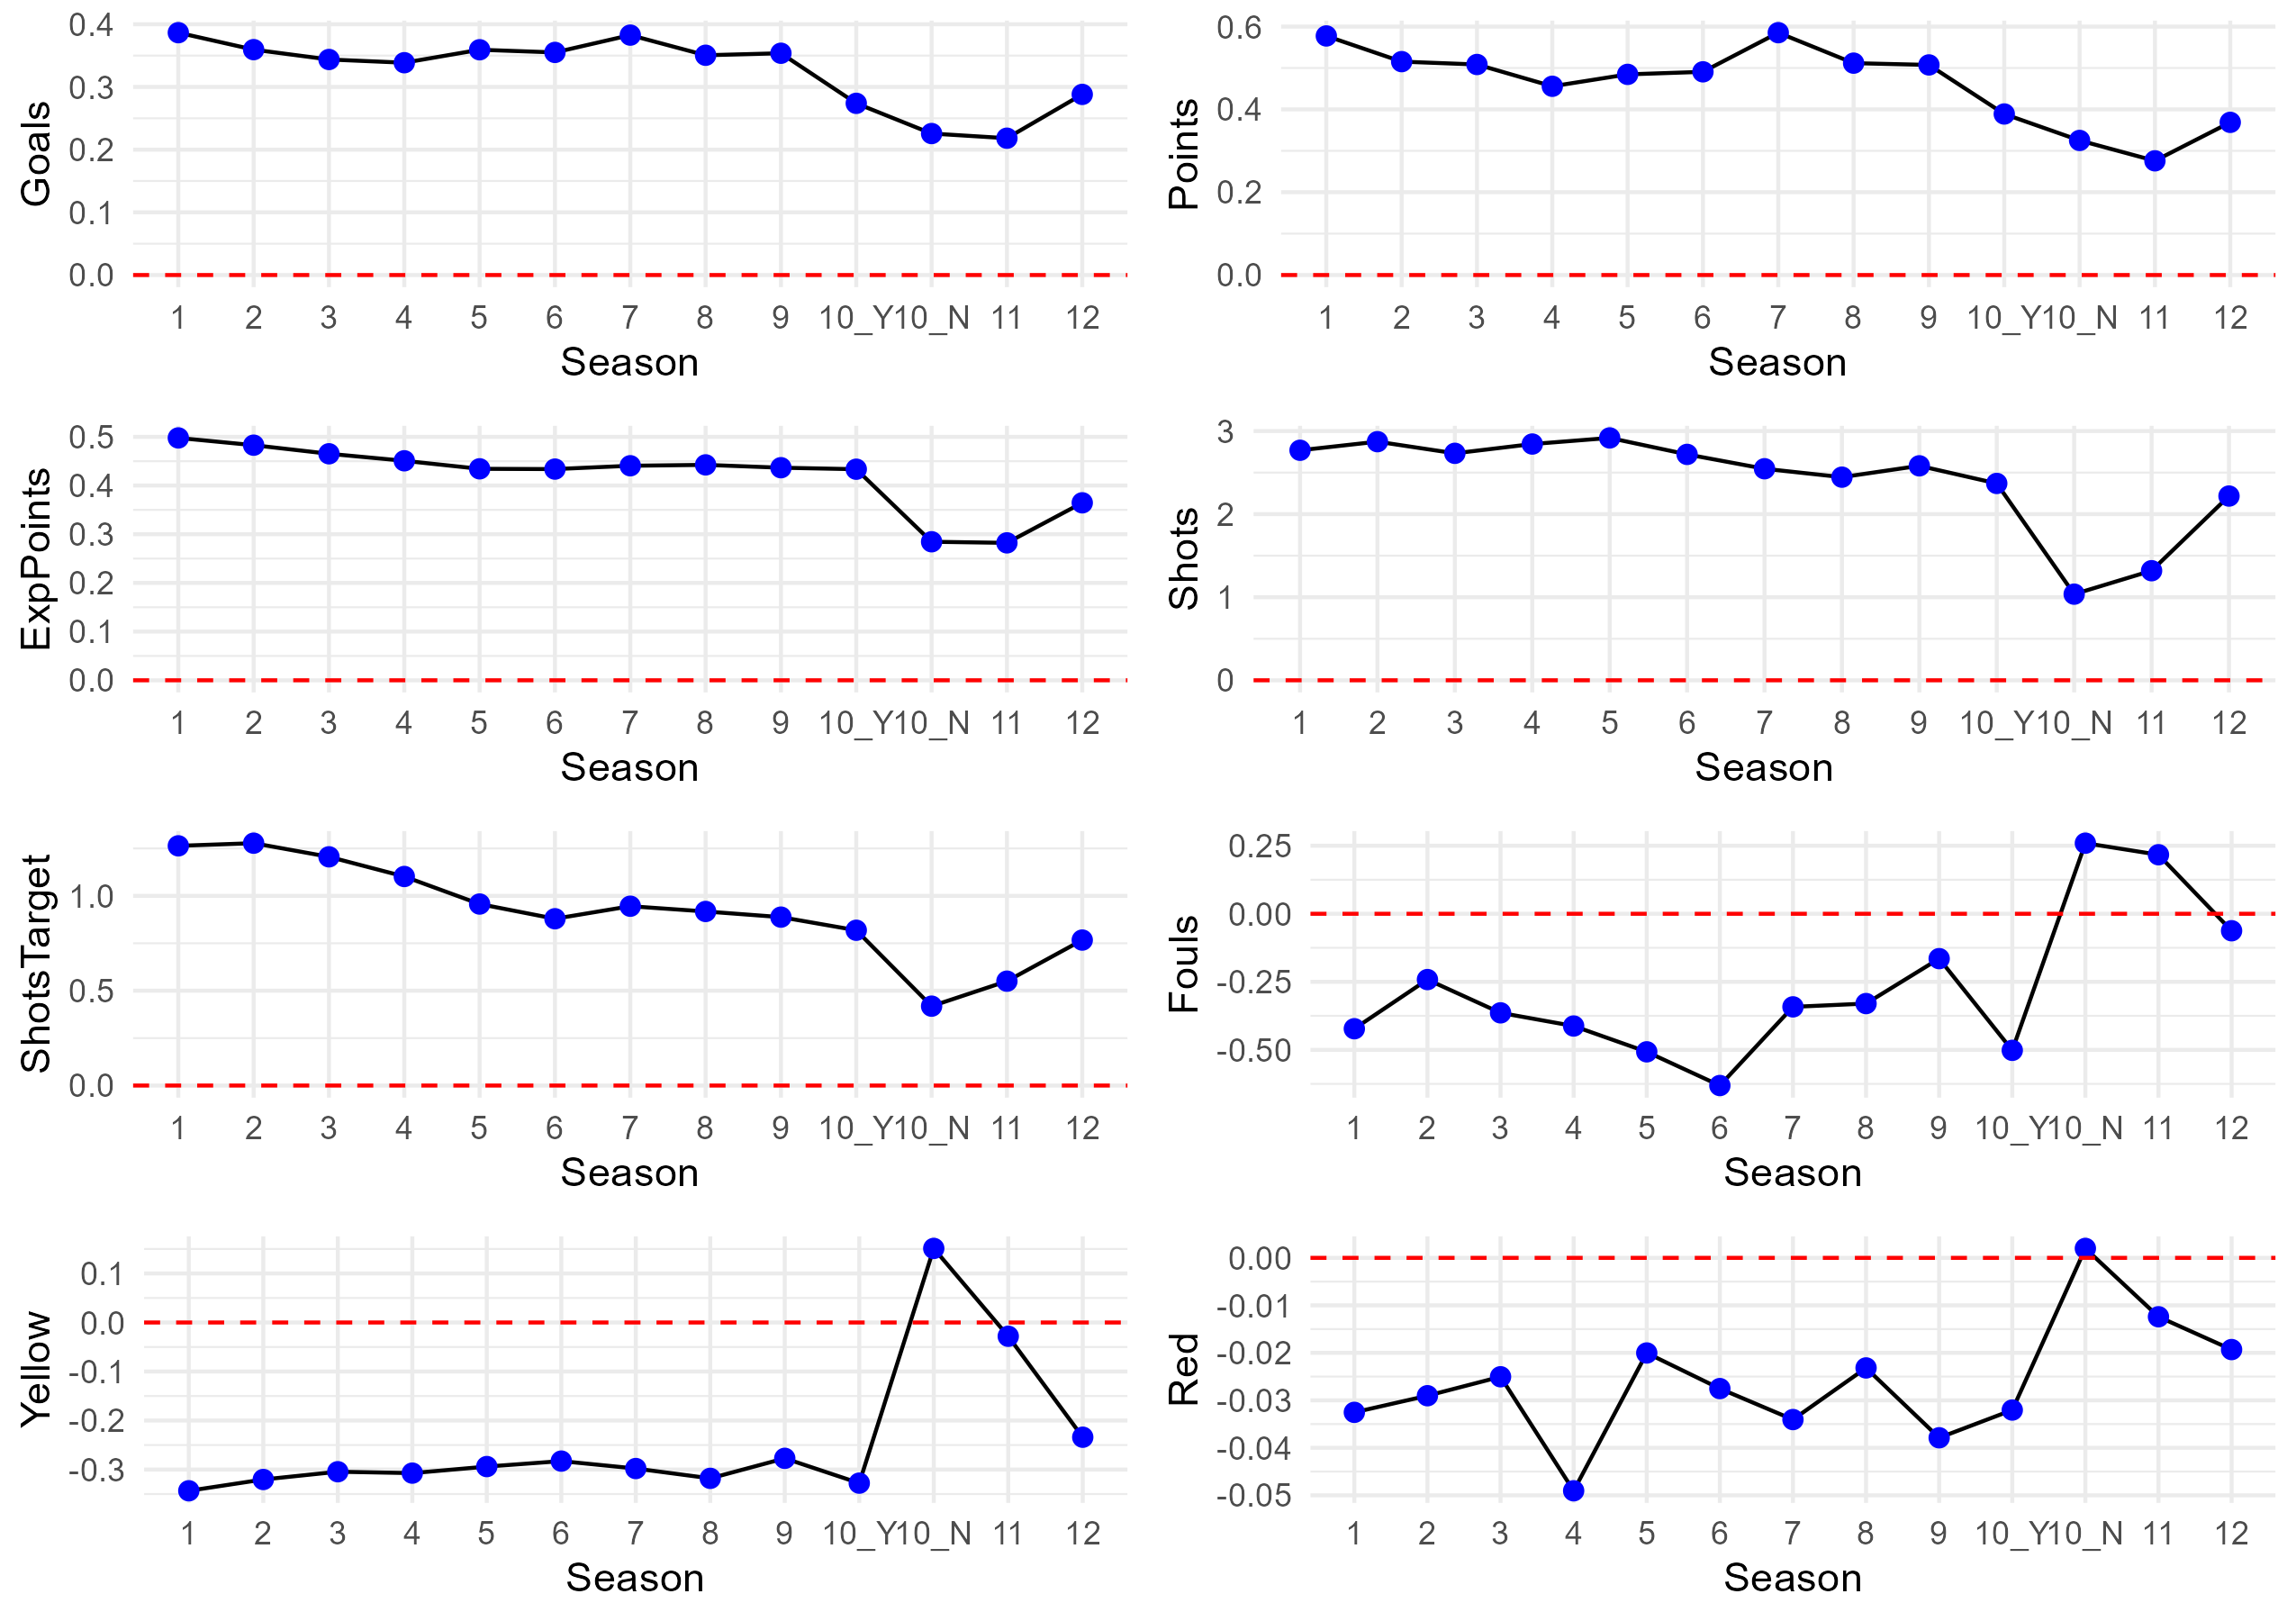
\includegraphics[width=1\textwidth]{Figures/Extended_plot.png}
    \label{fig:extend}
\end{figure}

\newpage

% NOTE
% FOR READABILITY I LET ALL TABLES HAVE A WIDER WIDTH THAN THE TEXT
% I at least limit it to be on both sides of the page

\begin{table}[H] \centering 
  \caption{Replication results over ten seasons for all dependent variables} 
  \label{tab:replic} 
  \addtolength{\leftskip} {-2cm}
  \addtolength{\rightskip}{-2cm}
\begin{tabular}{@{\extracolsep{5pt}}lD{.}{.}{-3} D{.}{.}{-3} D{.}{.}{-3} D{.}{.}{-3} } 
\\[-1.8ex]\hline 
\hline \\[-1.8ex] 
\\Difference H/A & \multicolumn{1}{c}{Goals} & \multicolumn{1}{c}{Points} & \multicolumn{1}{c}{Expected points} & \multicolumn{1}{c}{Shots} \\ 
\\[-1.8ex] & \multicolumn{1}{c}{(1)} & \multicolumn{1}{c}{(2)} & \multicolumn{1}{c}{(3)} & \multicolumn{1}{c}{(4)}\\ 
\hline \\[-1.8ex] 
  SpectatorsYes & 0.108 & 0.152 & 0.140^{***} & 1.406^{***} \\ 
  & (0.056) & (0.083) & (0.028) & (0.251) \\ 
  & & & & \\ 
 Season & -0.004 & -0.007 & -0.006^{***} & -0.045^{*} \\ 
  & (0.003) & (0.005) & (0.002) & (0.017) \\ 
  & & & & \\ 
 Constant & 0.224^{***} & 0.322^{***} & 0.280^{***} & 1.034^{***} \\ 
  & (0.055) & (0.081) & (0.029) & (0.243) \\ 
  & & & & \\ 
\hline \\[-1.8ex] 
$\sigma^2_{u}$ & \multicolumn{1}{c}{0.00} & \multicolumn{1}{c}{0.00} & \multicolumn{1}{c}{0.00} & \multicolumn{1}{c}{0.02} \\ 
$\sigma^2_{e}$ & \multicolumn{1}{c}{2.90} & \multicolumn{1}{c}{6.33} & \multicolumn{1}{c}{0.70} & \multicolumn{1}{c}{56.65} \\ 
Observations & \multicolumn{1}{c}{37,888} & \multicolumn{1}{c}{37,888} & \multicolumn{1}{c}{37,888} & \multicolumn{1}{c}{25,270} \\ 
Akaike Inf. Crit. & \multicolumn{1}{c}{147,903.700} & \multicolumn{1}{c}{177,432.700} & \multicolumn{1}{c}{94,139.760} & \multicolumn{1}{c}{173,741.500} \\ 
Bayesian Inf. Crit. & \multicolumn{1}{c}{147,946.400} & \multicolumn{1}{c}{177,475.500} & \multicolumn{1}{c}{94,182.470} & \multicolumn{1}{c}{173,782.200} \\ 
\hline 
\\Difference H/A & \multicolumn{1}{c}{Shots Target} & \multicolumn{1}{c}{Fouls} & \multicolumn{1}{c}{Yellow Cards} & \multicolumn{1}{c}{Red Cards} \\ 
\\[-1.8ex] & \multicolumn{1}{c}{(5)} & \multicolumn{1}{c}{(6)} & \multicolumn{1}{c}{(7)} & \multicolumn{1}{c}{(8)}\\ 
\hline \\[-1.8ex] 
 SpectatorsYes & 0.384^{**} & -0.589^{***} & -0.447^{***} & -0.033^{*} \\ 
  & (0.123) & (0.177) & (0.057) & (0.015) \\ 
  & & & & \\ 
 Season & -0.051^{***} & -0.009 & 0.003 & -0.0001 \\ 
  & (0.008) & (0.013) & (0.004) & (0.001) \\ 
  & & & & \\ 
 Constant & 0.418^{***} & 0.251 & 0.151^{**} & 0.002 \\ 
  & (0.118) & (0.198) & (0.055) & (0.014) \\ 
  & & & & \\ 
\hline \\[-1.8ex] 
$\sigma^2_{u}$ & \multicolumn{1}{c}{0.00} & \multicolumn{1}{c}{0.11} & \multicolumn{1}{c}{0.00} & \multicolumn{1}{c}{0.00} \\ 
$\sigma^2_{e}$ & \multicolumn{1}{c}{13.62} & \multicolumn{1}{c}{28.31} & \multicolumn{1}{c}{2.94} & \multicolumn{1}{c}{0.20} \\ 
Observations & \multicolumn{1}{c}{25,270} & \multicolumn{1}{c}{25,270} & \multicolumn{1}{c}{25,270} & \multicolumn{1}{c}{25,270} \\ 
Akaike Inf. Crit. & \multicolumn{1}{c}{137,729.600} & \multicolumn{1}{c}{156,230.800} & \multicolumn{1}{c}{98,962.080} & \multicolumn{1}{c}{31,171.130} \\ 
Bayesian Inf. Crit. & \multicolumn{1}{c}{137,770.300} & \multicolumn{1}{c}{156,271.500} & \multicolumn{1}{c}{99,002.770} & \multicolumn{1}{c}{31,211.810} \\ 
\hline 
\hline \\[-1.8ex] 
\textit{Note:}  & \multicolumn{4}{r}{$^{*}$p$<$0.05; $^{**}$p$<$0.01; $^{***}$p$<$0.001;} \\
& \multicolumn{4}{r}{$\sigma^2_{e}$ = Variance of first level residual error;}
& \multicolumn{5}{r}{$\sigma^2_{u}$ = Variance of second level residual error}
\end{tabular} 
\end{table} 

\begin{table}[H] \centering 
  \caption{Extended results over twelve seasons for all dependent variables}
  \label{tab:extend}
  \addtolength{\leftskip} {-2cm}
  \addtolength{\rightskip}{-2cm}
\begin{tabular}{@{\extracolsep{5pt}}lD{.}{.}{-3} D{.}{.}{-3} D{.}{.}{-3} D{.}{.}{-3} } 
\\[-1.8ex]\hline 
\hline \\[-1.8ex] 
\\ Difference H/A & \multicolumn{1}{c}{Goals} & \multicolumn{1}{c}{Points} & \multicolumn{1}{c}{Expected points} & \multicolumn{1}{c}{Shots} \\ 
\\[-1.8ex] & \multicolumn{1}{c}{(1)} & \multicolumn{1}{c}{(2)} & \multicolumn{1}{c}{(3)} & \multicolumn{1}{c}{(4)}\\ 
\hline \\[-1.8ex] 
 SpectatorsYes & 0.092^{**} & 0.145^{***} & 0.105^{***} & 0.996^{***} \\ 
  & (0.028) & (0.042) & (0.012) & (0.125) \\ 
  & & & & \\ 
 Season & -0.012^{***} & -0.019^{***} & -0.012^{***} & -0.084^{***} \\ 
  & (0.003) & (0.004) & (0.001) & (0.015) \\ 
  & & & & \\ 
 Constant & 0.061 & 0.071 & 0.125^{**} & 0.625^{**} \\ 
  & (0.044) & (0.064) & (0.048) & (0.199) \\ 
  & & & & \\ 
\hline \\[-1.8ex] 
$\sigma^2_{\upsilon}$ & \multicolumn{1}{c}{0.25} & \multicolumn{1}{c}{0.39} & \multicolumn{1}{c}{0.25} & \multicolumn{1}{c}{6.37} \\ 
$\sigma^2_{u}$ & \multicolumn{1}{c}{0.01} & \multicolumn{1}{c}{0.02} & \multicolumn{1}{c}{0.02} & \multicolumn{1}{c}{0.09} \\
$\sigma^2_{e}$ & \multicolumn{1}{c}{2.67} & \multicolumn{1}{c}{5.98} & \multicolumn{1}{c}{0.44} & \multicolumn{1}{c}{50.05} \\
Observations & \multicolumn{1}{c}{45,592} & \multicolumn{1}{c}{45,592} & \multicolumn{1}{c}{45,589} & \multicolumn{1}{c}{32,973} \\ 
Akaike Inf. Crit. & \multicolumn{1}{c}{175,114.400} & \multicolumn{1}{c}{211,776.900} & \multicolumn{1}{c}{94,092.890} & \multicolumn{1}{c}{223,438.800} \\ 
Bayesian Inf. Crit. & \multicolumn{1}{c}{175,166.800} & \multicolumn{1}{c}{211,829.300} & \multicolumn{1}{c}{94,145.260} & \multicolumn{1}{c}{223,489.300} \\ 
\hline 
\\Difference H/A & \multicolumn{1}{c}{Shots Target} & \multicolumn{1}{c}{Fouls} & \multicolumn{1}{c}{Yellow Cards} & \multicolumn{1}{c}{Red Cards} \\ 
\\[-1.8ex] & \multicolumn{1}{c}{(5)} & \multicolumn{1}{c}{(6)} & \multicolumn{1}{c}{(7)} & \multicolumn{1}{c}{(8)}\\ 
\hline \\[-1.8ex] 
 SpectatorsYes & 0.245^{***} & -0.402^{***} & -0.279^{***} & -0.018^{*} \\ 
  & (0.061) & (0.091) & (0.030) & (0.008) \\ 
  & & & & \\ 
 Season & -0.063^{***} & 0.028^{**} & 0.007 & 0.001 \\ 
  & (0.007) & (0.011) & (0.003) & (0.001) \\ 
  & & & & \\ 
 Constant & 0.145 & 0.255 & 0.041 & -0.008 \\ 
  & (0.101) & (0.136) & (0.032) & (0.007) \\ 
  & & & & \\ 
\hline \\[-1.8ex] 
$\sigma^2_{\upsilon}$ & \multicolumn{1}{c}{1.39} & \multicolumn{1}{c}{1.29} & \multicolumn{1}{c}{0.07} & \multicolumn{1}{c}{0.00} \\ 
$\sigma^2_{u}$ & \multicolumn{1}{c}{0.03} & \multicolumn{1}{c}{0.08} & \multicolumn{1}{c}{0.00} & \multicolumn{1}{c}{0.00} \\
$\sigma^2_{e}$ & \multicolumn{1}{c}{11.85} & \multicolumn{1}{c}{27.29} & \multicolumn{1}{c}{2.93} & \multicolumn{1}{c}{0.20} \\
Observations & \multicolumn{1}{c}{32,973} & \multicolumn{1}{c}{32,973} & \multicolumn{1}{c}{32,973} & \multicolumn{1}{c}{32,973} \\ 
Akaike Inf. Crit. & \multicolumn{1}{c}{175,913.300} & \multicolumn{1}{c}{203,158.900} & \multicolumn{1}{c}{129,429.800} & \multicolumn{1}{c}{40,881.940} \\ 
Bayesian Inf. Crit. & \multicolumn{1}{c}{175,963.700} & \multicolumn{1}{c}{203,209.300} & \multicolumn{1}{c}{129,480.200} & \multicolumn{1}{c}{40,932.360} \\ 
\hline 
\hline \\[-1.8ex] 
\textit{Note:}  & \multicolumn{4}{r}{$^{*}$p$<$0.05; $^{**}$p$<$0.01; $^{***}$p$<$0.001;} \\
& \multicolumn{4}{r}{$\sigma^2_{e}$ = Variance of first level residual error;}
& \multicolumn{5}{r}{$\sigma^2_{u}$ = Variance of second level residual error;}
& \multicolumn{5}{r}{$\sigma^2_{\upsilon}$ = Variance of third level residual error}
\end{tabular} 
\end{table} 

\begin{table}[H] \centering 
  \caption{Exploratory results over twelve Premier League seasons for all dependent variables}
  \label{tab:explor} 
  \addtolength{\leftskip} {-2cm}
  \addtolength{\rightskip}{-2cm}
\begin{tabular}{@{\extracolsep{5pt}}lD{.}{.}{-3} D{.}{.}{-3} D{.}{.}{-3} D{.}{.}{-3} } 
\\[-1.8ex]\hline 
\hline \\[-1.8ex] 
\\ Difference H/A & \multicolumn{1}{c}{Goals} & \multicolumn{1}{c}{Points} & \multicolumn{1}{c}{Expected points} & \multicolumn{1}{c}{Shots} \\ 
\\[-1.8ex] & \multicolumn{1}{c}{(1)} & \multicolumn{1}{c}{(2)} & \multicolumn{1}{c}{(3)} & \multicolumn{1}{c}{(4)}\\ 
\hline \\[-1.8ex] 
 Occupancy & 0.267^{**} & 0.447^{**} & 0.146^{**} & 1.500^{***} \\ 
  & (0.098) & (0.138) & (0.047) & (0.446) \\ 
  & & & & \\ 
 Season\_c & -0.021^{*} & -0.028^{*} & -0.022^{***} & -0.118^{**} \\ 
  & (0.009) & (0.013) & (0.004) & (0.042) \\ 
  & & & & \\ 
 Constant & -0.276^{*} & -0.419^{*} & -0.117 & -0.649 \\ 
  & (0.127) & (0.165) & (0.108) & (0.670) \\ 
  & & & & \\ 
\hline \\[-1.8ex] 
$\sigma^2_{u}$ & \multicolumn{1}{c}{0.34} & \multicolumn{1}{c}{0.50} & \multicolumn{1}{c}{0.38} & \multicolumn{1}{c}{11.32} \\ 
$\sigma^2_{e}$ & \multicolumn{1}{c}{3.01} & \multicolumn{1}{c}{6.01} & \multicolumn{1}{c}{0.68} & \multicolumn{1}{c}{62.53} \\ 
Observations & \multicolumn{1}{c}{4,558} & \multicolumn{1}{c}{4,558} & \multicolumn{1}{c}{4,558} & \multicolumn{1}{c}{4,558} \\ 
Log Likelihood & \multicolumn{1}{c}{-9,023.024} & \multicolumn{1}{c}{-10,594.960} & \multicolumn{1}{c}{-5,670.078} & \multicolumn{1}{c}{-15,947.010} \\ 
Akaike Inf. Crit. & \multicolumn{1}{c}{18,056.050} & \multicolumn{1}{c}{21,199.910} & \multicolumn{1}{c}{11,350.160} & \multicolumn{1}{c}{31,904.010} \\ 
Bayesian Inf. Crit. & \multicolumn{1}{c}{18,088.170} & \multicolumn{1}{c}{21,232.040} & \multicolumn{1}{c}{11,382.280} & \multicolumn{1}{c}{31,936.140} \\ 
\hline 
\\Difference H/A & \multicolumn{1}{c}{Shots Target} & \multicolumn{1}{c}{Fouls} & \multicolumn{1}{c}{Yellow Cards} & \multicolumn{1}{c}{Red Cards} \\ 
\\[-1.8ex] & \multicolumn{1}{c}{(5)} & \multicolumn{1}{c}{(6)} & \multicolumn{1}{c}{(7)} & \multicolumn{1}{c}{(8)}\\ 
\hline \\[-1.8ex] 
 Occupancy & 0.291 & -0.893^{***} & -0.101 & -0.014 \\ 
  & (0.219) & (0.256) & (0.087) & (0.020) \\ 
  & & & & \\ 
 Season\_c & -0.150^{***} & 0.005 & 0.029^{***} & 0.001 \\ 
  & (0.021) & (0.024) & (0.008) & (0.002) \\ 
  & & & & \\ 
 Constant & -0.798^{*} & 0.545^{*} & 0.072 & -0.004 \\ 
  & (0.336) & (0.272) & (0.085) & (0.017) \\ 
  & & & & \\ 
\hline \\[-1.8ex] 
$\sigma^2_{u}$ & \multicolumn{1}{c}{2.90} & \multicolumn{1}{c}{0.96} & \multicolumn{1}{c}{0.06} & \multicolumn{1}{c}{0.00} \\ 
$\sigma^2_{e}$ & \multicolumn{1}{c}{15.14} & \multicolumn{1}{c}{20.93} & \multicolumn{1}{c}{2.44} & \multicolumn{1}{c}{0.13} \\ 
Observations & \multicolumn{1}{c}{4,558} & \multicolumn{1}{c}{4,558} & \multicolumn{1}{c}{4,558} & \multicolumn{1}{c}{4,558} \\ 
Log Likelihood & \multicolumn{1}{c}{-12,715.650} & \multicolumn{1}{c}{-13,430.670} & \multicolumn{1}{c}{-8,527.484} & \multicolumn{1}{c}{-1,894.340} \\ 
Akaike Inf. Crit. & \multicolumn{1}{c}{25,441.290} & \multicolumn{1}{c}{26,871.350} & \multicolumn{1}{c}{17,064.970} & \multicolumn{1}{c}{3,798.679} \\ 
Bayesian Inf. Crit. & \multicolumn{1}{c}{25,473.410} & \multicolumn{1}{c}{26,903.470} & \multicolumn{1}{c}{17,097.090} & \multicolumn{1}{c}{3,830.803} \\   
\hline 
\hline \\[-1.8ex] 
\textit{Note:}  & \multicolumn{4}{r}{$^{*}$p$<$0.05; $^{**}$p$<$0.01; $^{***}$p$<$0.001;} \\
& \multicolumn{4}{r}{$\sigma^2_{e}$ = Variance of first level residual error;}
& \multicolumn{5}{r}{$\sigma^2_{u}$ = Variance of second level residual error}
\end{tabular} 
\end{table} 

\newpage

\section{Discussion}

This report investigates the impact of spectator attendance on the home advantage in professional European football leagues by replicating and extending a peer-reviewed study that analyzed a series of ghost games played during the COVID-19 pandemic from March 2020 in a natural experiment. This report successfully replicated the study by Wunderlich et al. (2021) \cite{wunderlich2021does} and extended the original study with additional modeling and the inclusion of more recent data. The main finding of this report is that the home advantage decreases in the absence of an audience. Therefore, successfully validating the initial effect investigated by the replicated study. This can be observed in the categories  of disciplinary sanctions (fouls, yellow cards, red cards), match dominance (shots, shots on target), market expectation (betting odds), and also match results (goals, points). In particular, the findings on match results are of key interest, as they contradict the results of Wunderlich et al. (2021) \cite{wunderlich2021does}. Their findings state that home teams receive fewer disciplinary sanctions and are able to create more offensive actions compared to the away teams. However, these differences between home and away teams do not translate into a home advantage in terms of more points won or more goals scored.  

A possible reason for these discrepant results is that the replicated study had highly unbalanced data and used a small set of actual ghost games played (N = 1,006) compared to games with spectators (N = 36,882). The extension included more games in the absence of spectators (N = 4,878), which supports balancing the classes (N = 40,714). 
In addition, the extension includes the first season after the COVID-19 pandemic with readmitted spectators. This provides an opportunity to see if home advantage increases again when spectators return to the stadium. From the visual inspection of Figure \ref{fig:extend} it can be concluded that the home advantage indeed increases again for all dependent variables. However, a decreasing home advantage over the seasons is observed for most dependent variables as can be seen in Table \ref{tab:extend}. An alternative explanation could be the model changes made to account for the hierarchical structure of the data. The ICC must be considered when using random effects as it indicates the variation in the outcome variables accounted for by the cluster structure of the data. The ICC of the three-level hierarchical structure of matches played by a given home team, in a given division, warranted the use of random effects. However, the hierarchical structure of matches in a given division applied in the replicated study did not justify the need for a hierarchical structure based on the ICC.

This report also focuses on additional exploratory analyses. This approach is based on the idea that the binary classification of games with spectators and games without spectators leads to a significant loss of information. The inclusion of the occupancy rate is intended to overcome the loss of information, as it is a continuous variable that has varying values even within seasons. This approach is of key interest for the 2021/2022 season, as capacity was limited to a fixed spectator size for several games. However, the exploratory analysis was based exclusively on Premier League data, as data for other divisions is scarce.

Potential future research with this data set could examine whether bookmakers set their betting odds correctly during the COVID-19 pandemic, as this report showed a decline in home team advantage that should have been accounted for. Considering the differences in points per game as the dependent variable, expected points as the independent variable would be expected to be around the value of 1, as an increase in expected points should exactly match the actual increase in points. Coefficients greater or less than one would indicate deviations from efficiency. 

A limitation of this study is the absence of potential confounding variables. In particular, with observational data, it is difficult to control for variables of interest since the data is not collected in an experimental setting. Therefore, many other variables could confound the results and should be considered in the analysis. Several studies that investigated related effects considered variables such as a team's market value, points scored in the four games prior to the game in question, and a team's standings \cite{mccarrick2021home,cross2020fans,ponzo2018does,jimenez2021home}. All of these variables appear to have a significant impact on the outcome of the game, and to establish a causal relationship between spectator attendance and home team advantage, all confounding variables must be accounted for. Obtaining this type of information often requires additional data collection, which is costly in terms of time and money. Nevertheless, to achieve the goal of causality, these additional steps should be considered.

\section{Conclusion}
In this report, an existing peer-reviewed study examining a series of ghost games during the COVID-19 pandemic in a natural experiment was successfully replicated and extended. New insights were gained regarding the impact of spectator absence on actual game outcomes, which contradicted the results of the replicated study. Additional findings resulted from the inclusion of new variables in the model, as well as the inclusion of the 2021/2022 season to show the impact after the COVID-19 pandemic when spectators were readmitted. This report also discusses exploratory analyses and the advantages and disadvantages of using an open-source observational data set. 

